\ifdefined\withimages
  \newpage
  \tikz[remember picture,overlay] \node[opacity=1,inner sep=0pt] at (current page.center){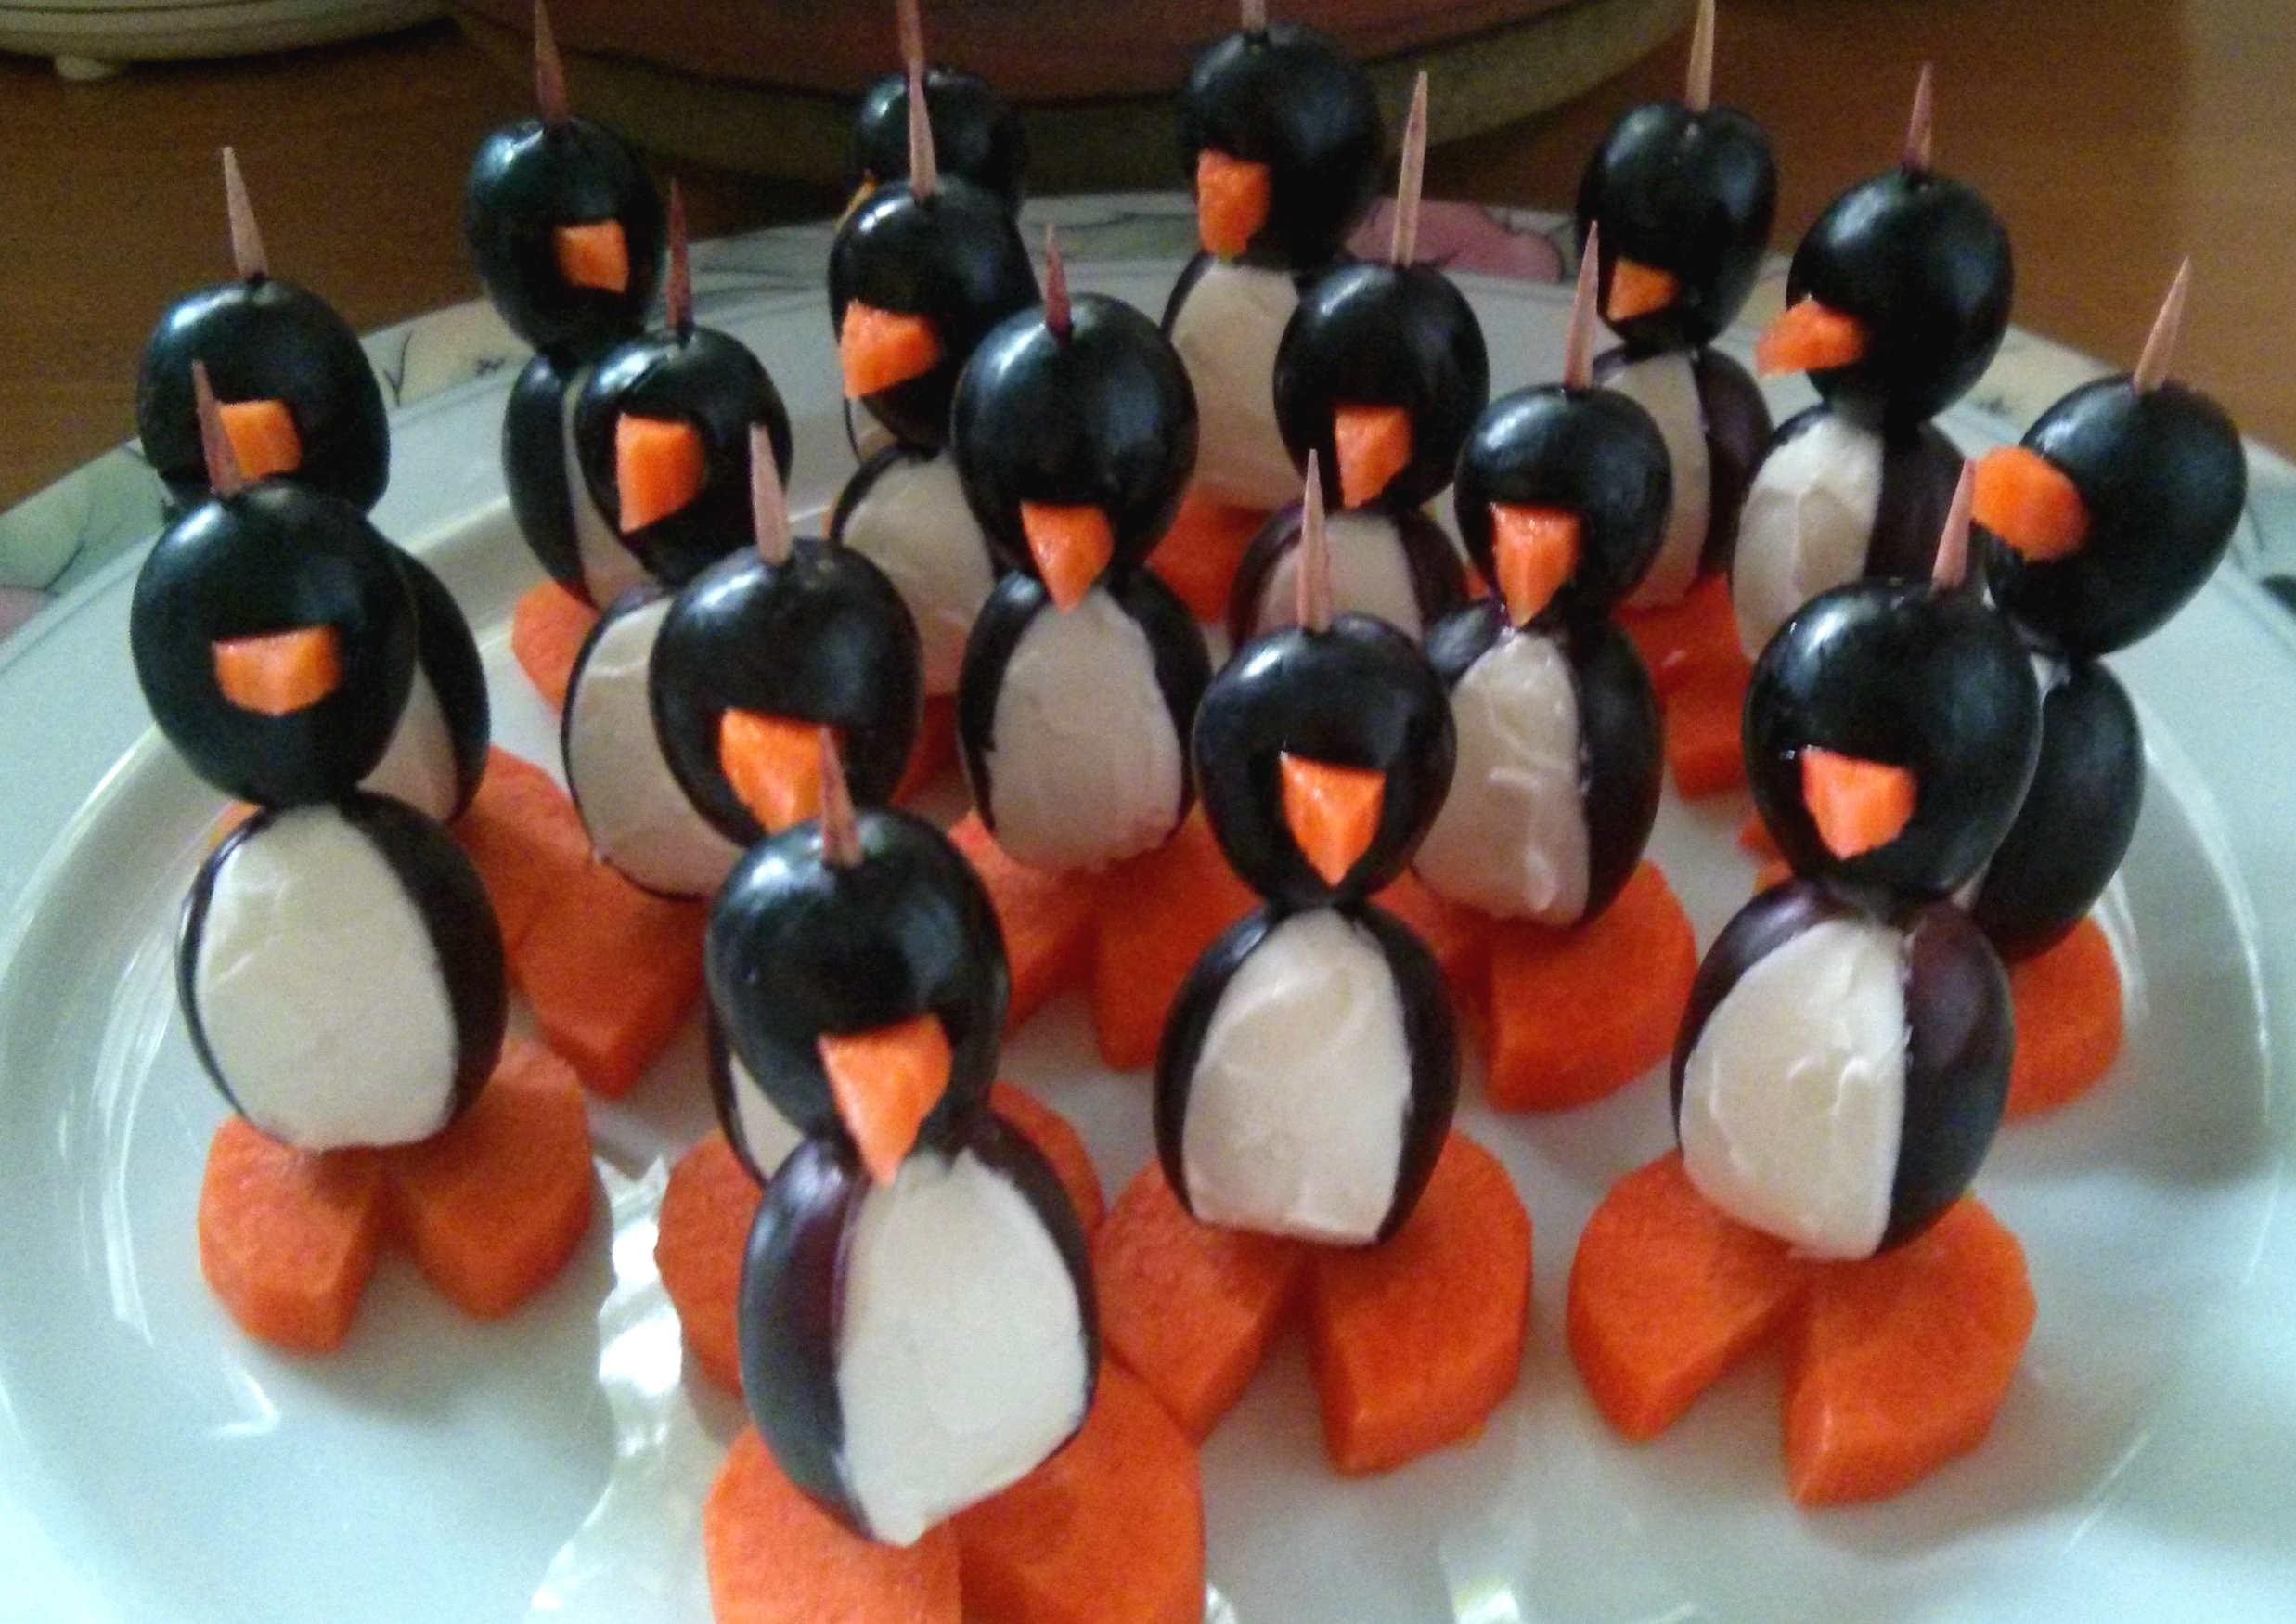
\includegraphics[width=\paperwidth,height=\paperheight]{./bilder/pinguine_ratio.jpg}};
\fi

\begin{recipe}[]{Pinguine} %Quelle
  \timerecipe[Minuten]{ca. 30} %mit [EINHEIT]
  \personcount[Stück]{10} % mit[ART]
	\ingredient{1 Karotte} % ggf. \nicefrac{1}{2}
	\ingredient{20 dunkle Weintrauben}
	\ingredient{200g Frischkäse}
	\ingredient{10 Zahnstocher}

\step
\textbf{1 Karotte} in drei bis vier Millimeter dicke Scheibchen schneiden. Aus den Möhrenscheibchen mit je zwei Schnitten bis zur Mitte ein kleines Dreieck herausschneiden. Dreieck beiseitelegen (ergibt den Schnabel des Pinguins). 

\step
In eine \textbf{kleinere rote Traube} einen sehr kleinen Schlitz für den Schnabel schneiden und die Möhrenecke einstecken. Aus einer \textbf{größeren Traube} ein Drittel als Spalte ausschneiden. 

\step
Den entstandenen Spalt sauber mit \textbf{Frischkäse} füllen (das gibt den Pinguinbauch). Die beiden Trauben auf einen Zahnstocher stecken (die kleine als Kopf oben, die große als Bauch unten) und unten die Karotten-Füße befestigen.

%\tippbox{\textbf{Tipp:} ...} % Tipp in extra Rahmen
\end{recipe}